
    \documentclass{article}
    \usepackage{amsmath, amssymb}
    \usepackage[T2A]{fontenc} % Cyrillic font encoding
    \usepackage[utf8]{inputenc} % UTF-8 input encoding
    \usepackage{paratype} % PT Serif/Sans fonts with good Cyrillic support
    \usepackage[ukrainian]{babel} % Ukrainian language support
    \usepackage[a4paper, margin=2.5cm]{geometry}
    \usepackage{mathtools}
    \usepackage{xcolor}
    \usepackage{graphicx}
    \usepackage{float}
    \usepackage{enumitem}
    \usepackage{tikz}
    \usetikzlibrary{matrix}
    \usepackage{amsthm}
    \usepackage{booktabs}
    \usepackage{fancyhdr}
    \usepackage{titlesec}
    \usepackage{array}
    \usepackage{longtable}
    \usepackage{siunitx}

    \titleformat{\section}{\Large\bfseries}{\thesection}{1em}{}
    \titleformat{\subsection}{\large\bfseries}{\thesubsection}{1em}{}

    \pagestyle{fancy}
    \fancyhf{}
    \fancyhead[C]{\textbf{Звіт багатофакторної лінійної регресії}}
    \fancyfoot[C]{\thepage}
    \renewcommand{\headrulewidth}{0.4pt}

    \begin{document}

    \begin{center}
    \Large\textbf{Звіт багатофакторної лінійної регресії}
    \end{center}

    \vspace{1cm}

    \textbf{Дата:} \today

    \vspace{0.5cm}

    \section{Опис моделі}

    \begin{itemize}
        \item Залежна змінна: \textbf{MEDV}
        \item Незалежні змінні: \textbf{CHAS, NOX, RM}
        \item Коефіцієнт детермінації $R^2$: \textbf{0.5537}
        \item Середньоквадратична похибка: \textbf{37.6753}
    \end{itemize}

    \vspace{0.5cm}

    \section{Коефіцієнти регресії}

    \begin{center}
    \begin{tabular}{lcccc}
    \toprule
    \textbf{Змінна} & \textbf{Коефіцієнт} & \textbf{P-значення} & \textbf{Значущість (p < 0.05)} \\
    \midrule
    Вільний член & -16.3270 & Н/Д & Н/Д \\
    CHAS & 5.0253 & 0.0000 & Так \\
NOX & -20.2150 & 0.0000 & Так \\
RM & 7.9116 & 0.0000 & Так \\

    \bottomrule
    \end{tabular}
    \end{center}

    \vspace{1cm}
    
    \begin{figure}[H]
        \centering
        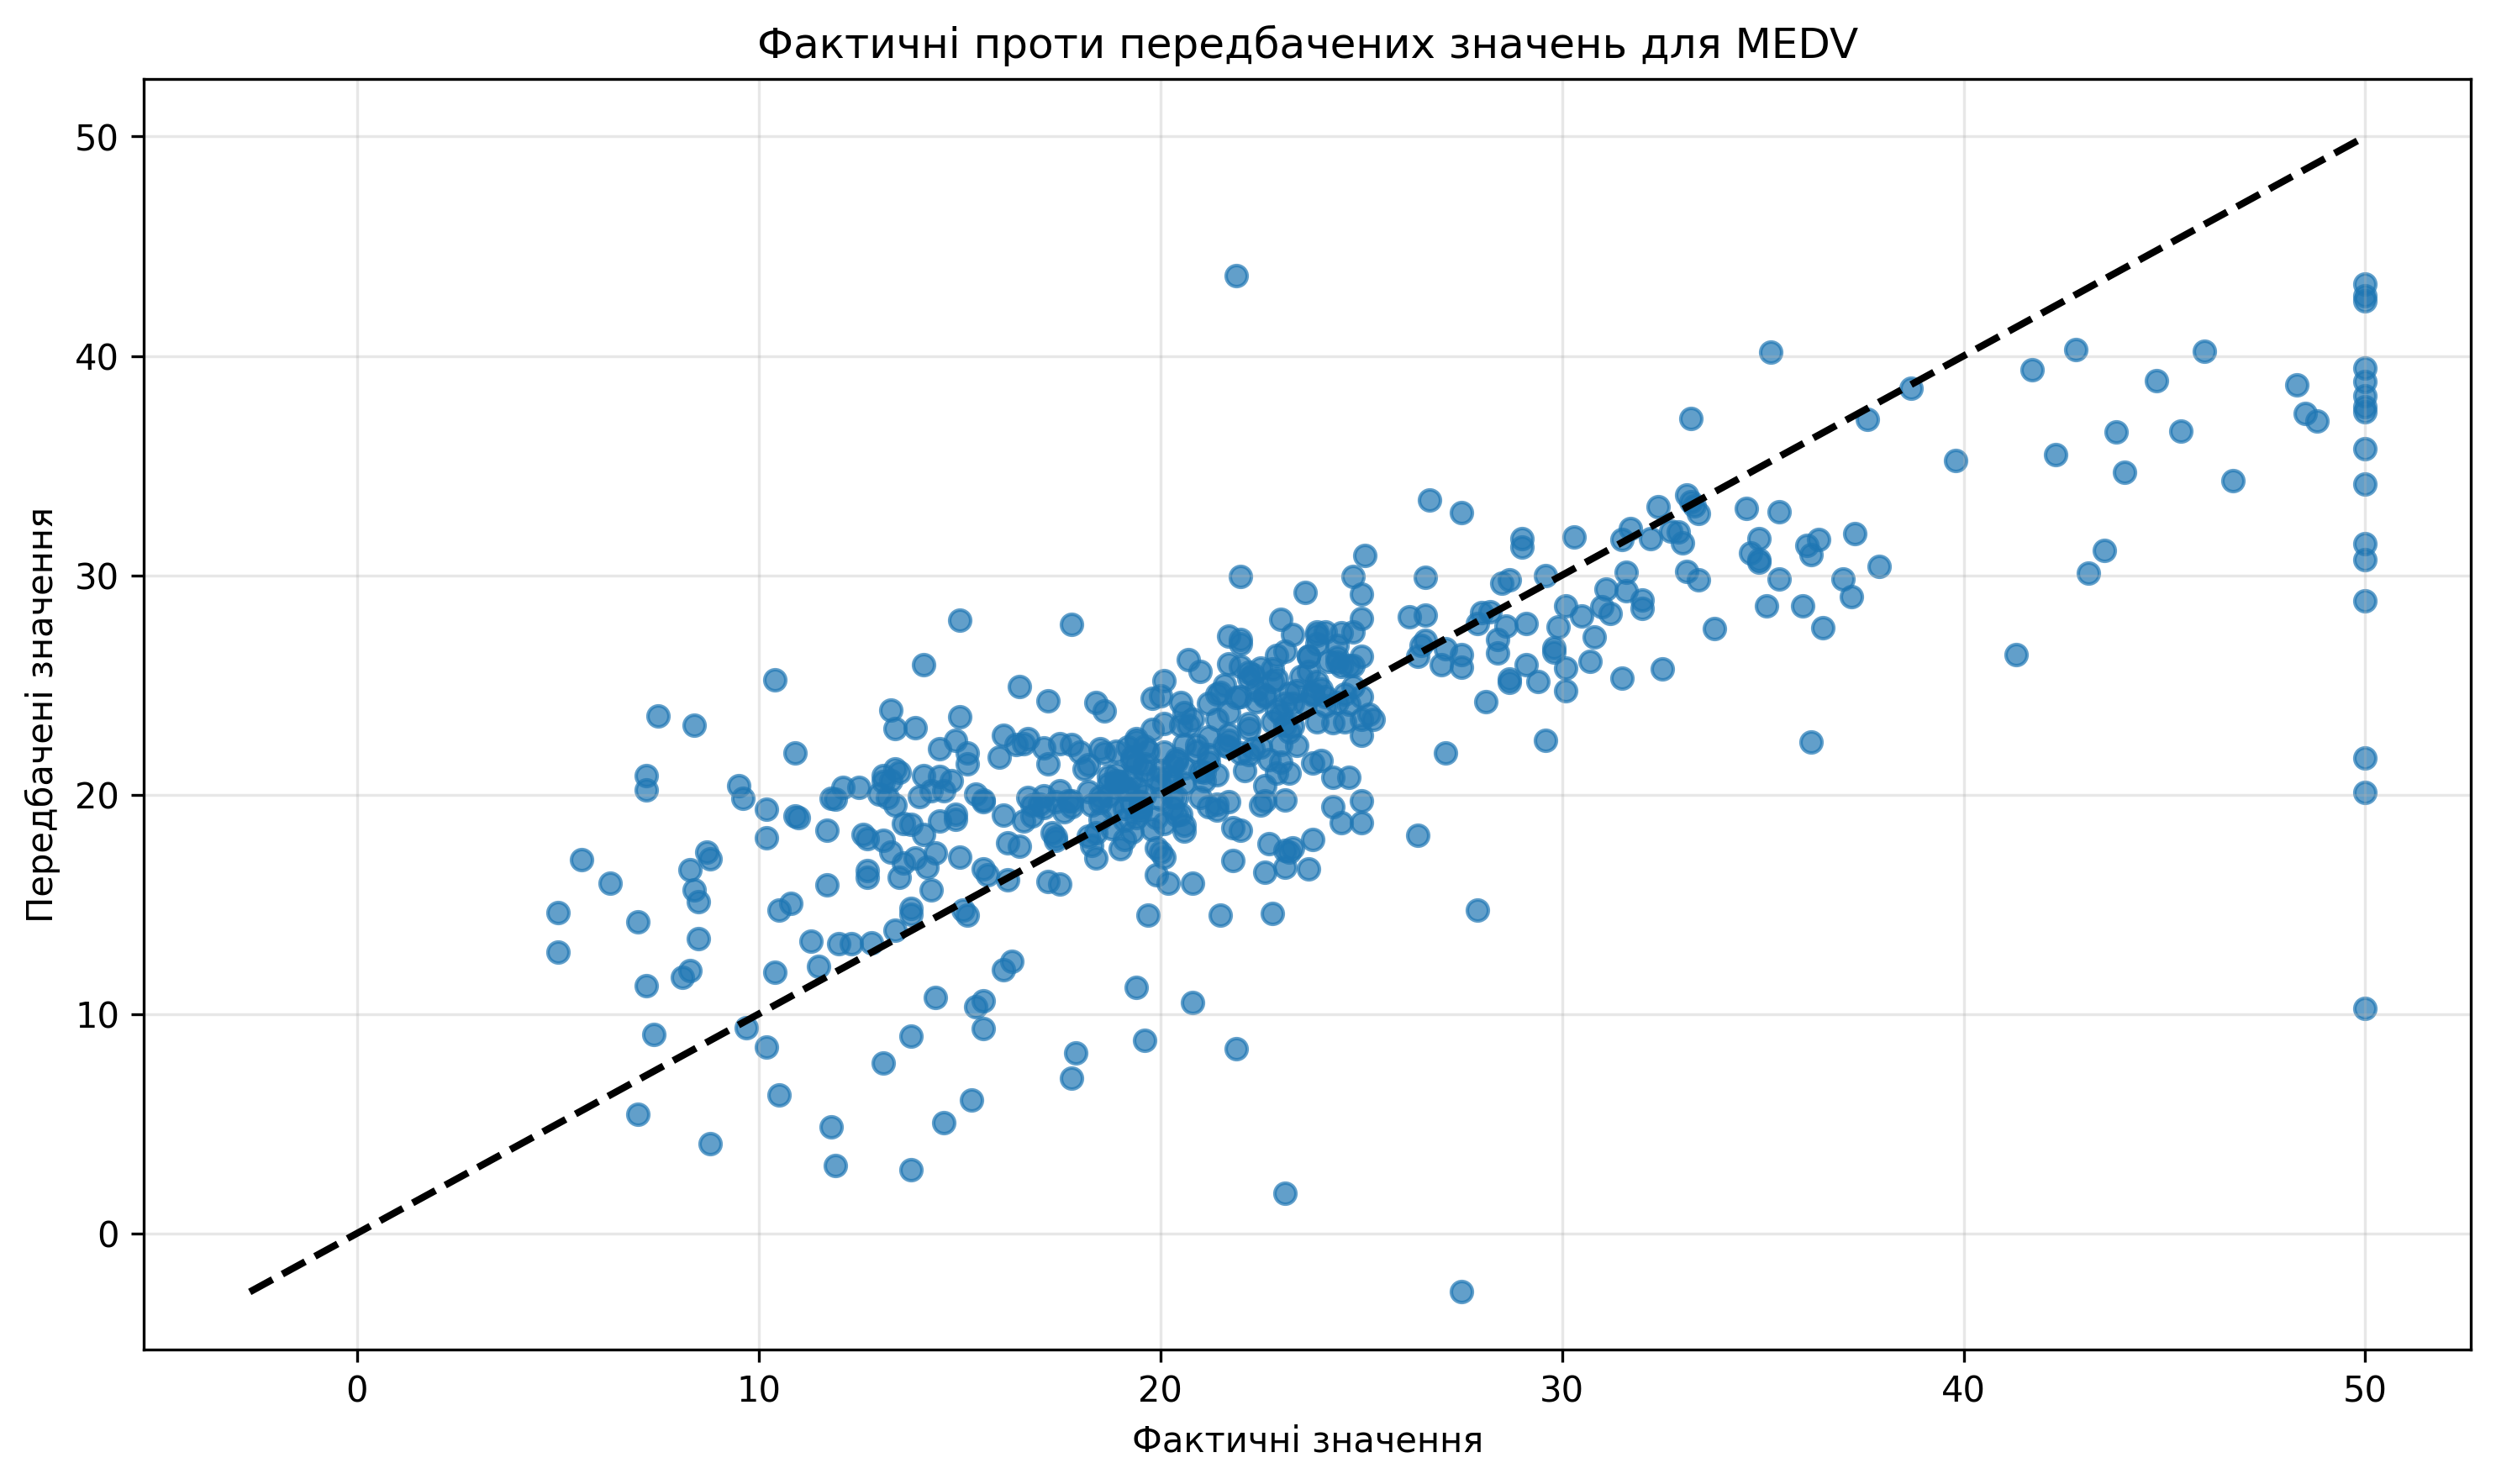
\includegraphics[width=0.8\textwidth]{actual_vs_predicted.png}
        \caption{Фактичні проти передбачених значень}
        \label{fig:фактичні_проти_передбачених_значень}
    \end{figure}

    \vspace{0.5cm}
    
    \begin{figure}[H]
        \centering
        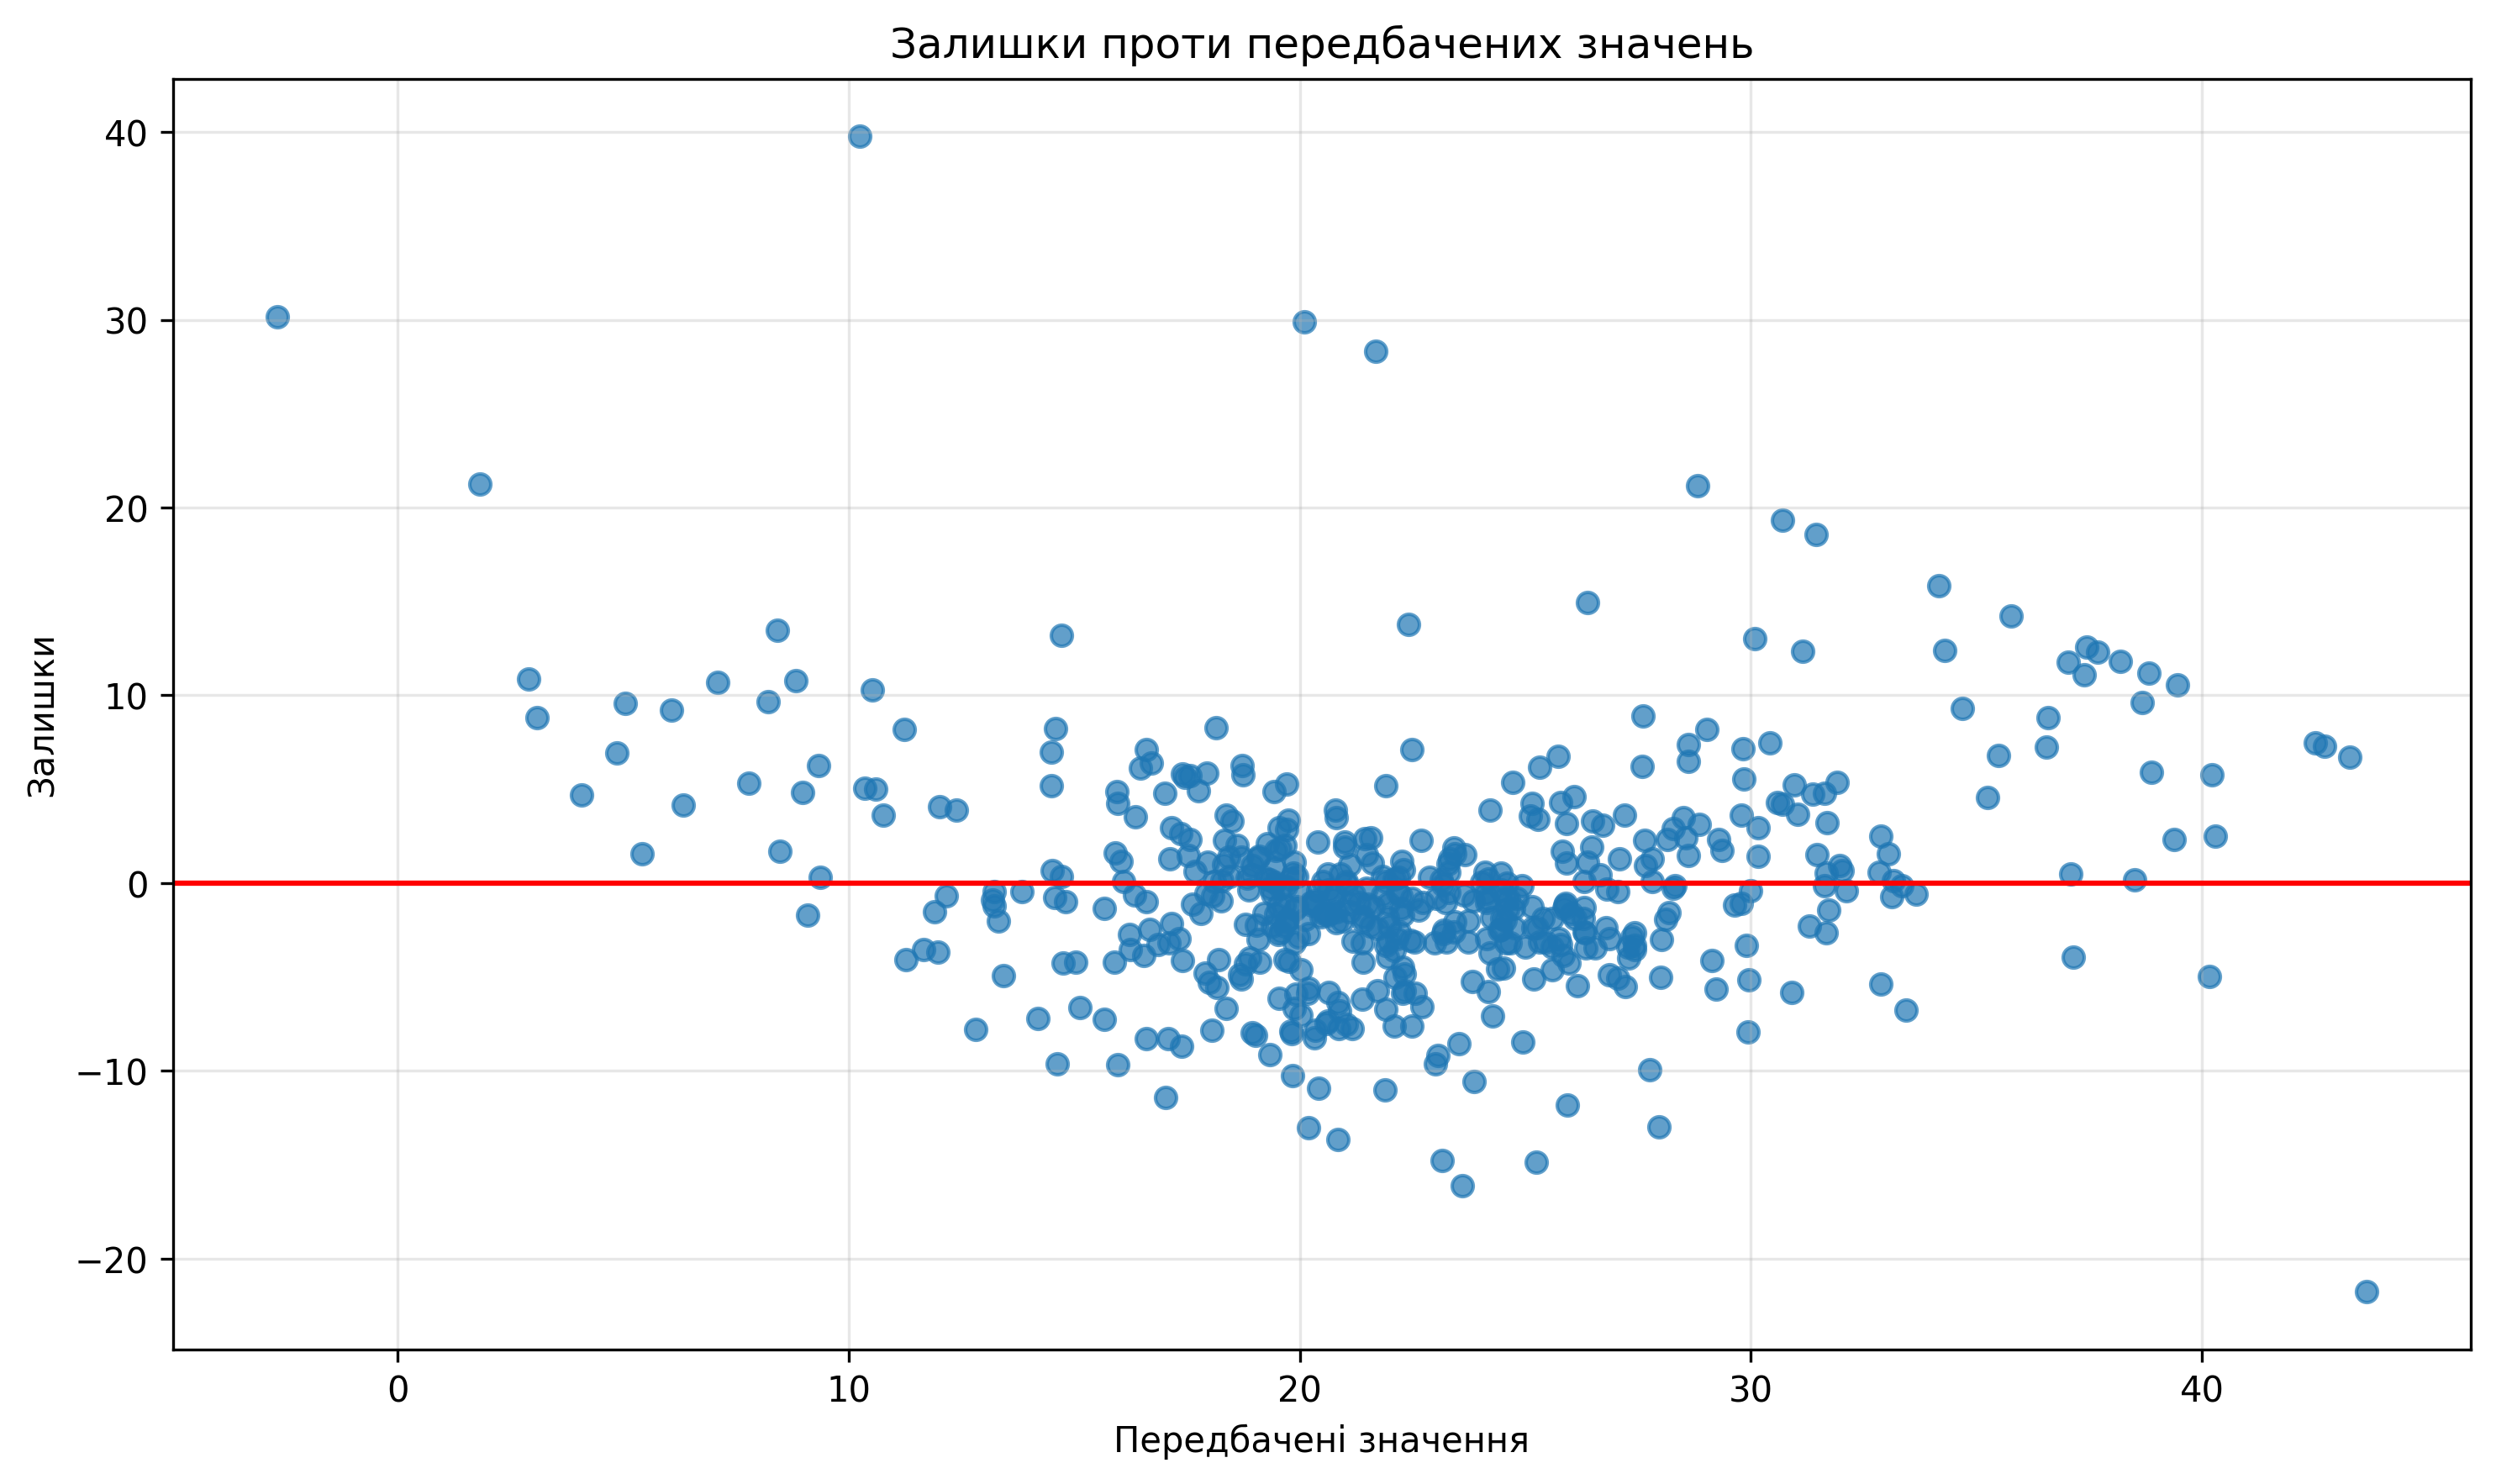
\includegraphics[width=0.8\textwidth]{residuals.png}
        \caption{Графік залишків}
        \label{fig:графік_залишків}
    \end{figure}

    \vspace{0.5cm}
    
    \begin{figure}[H]
        \centering
        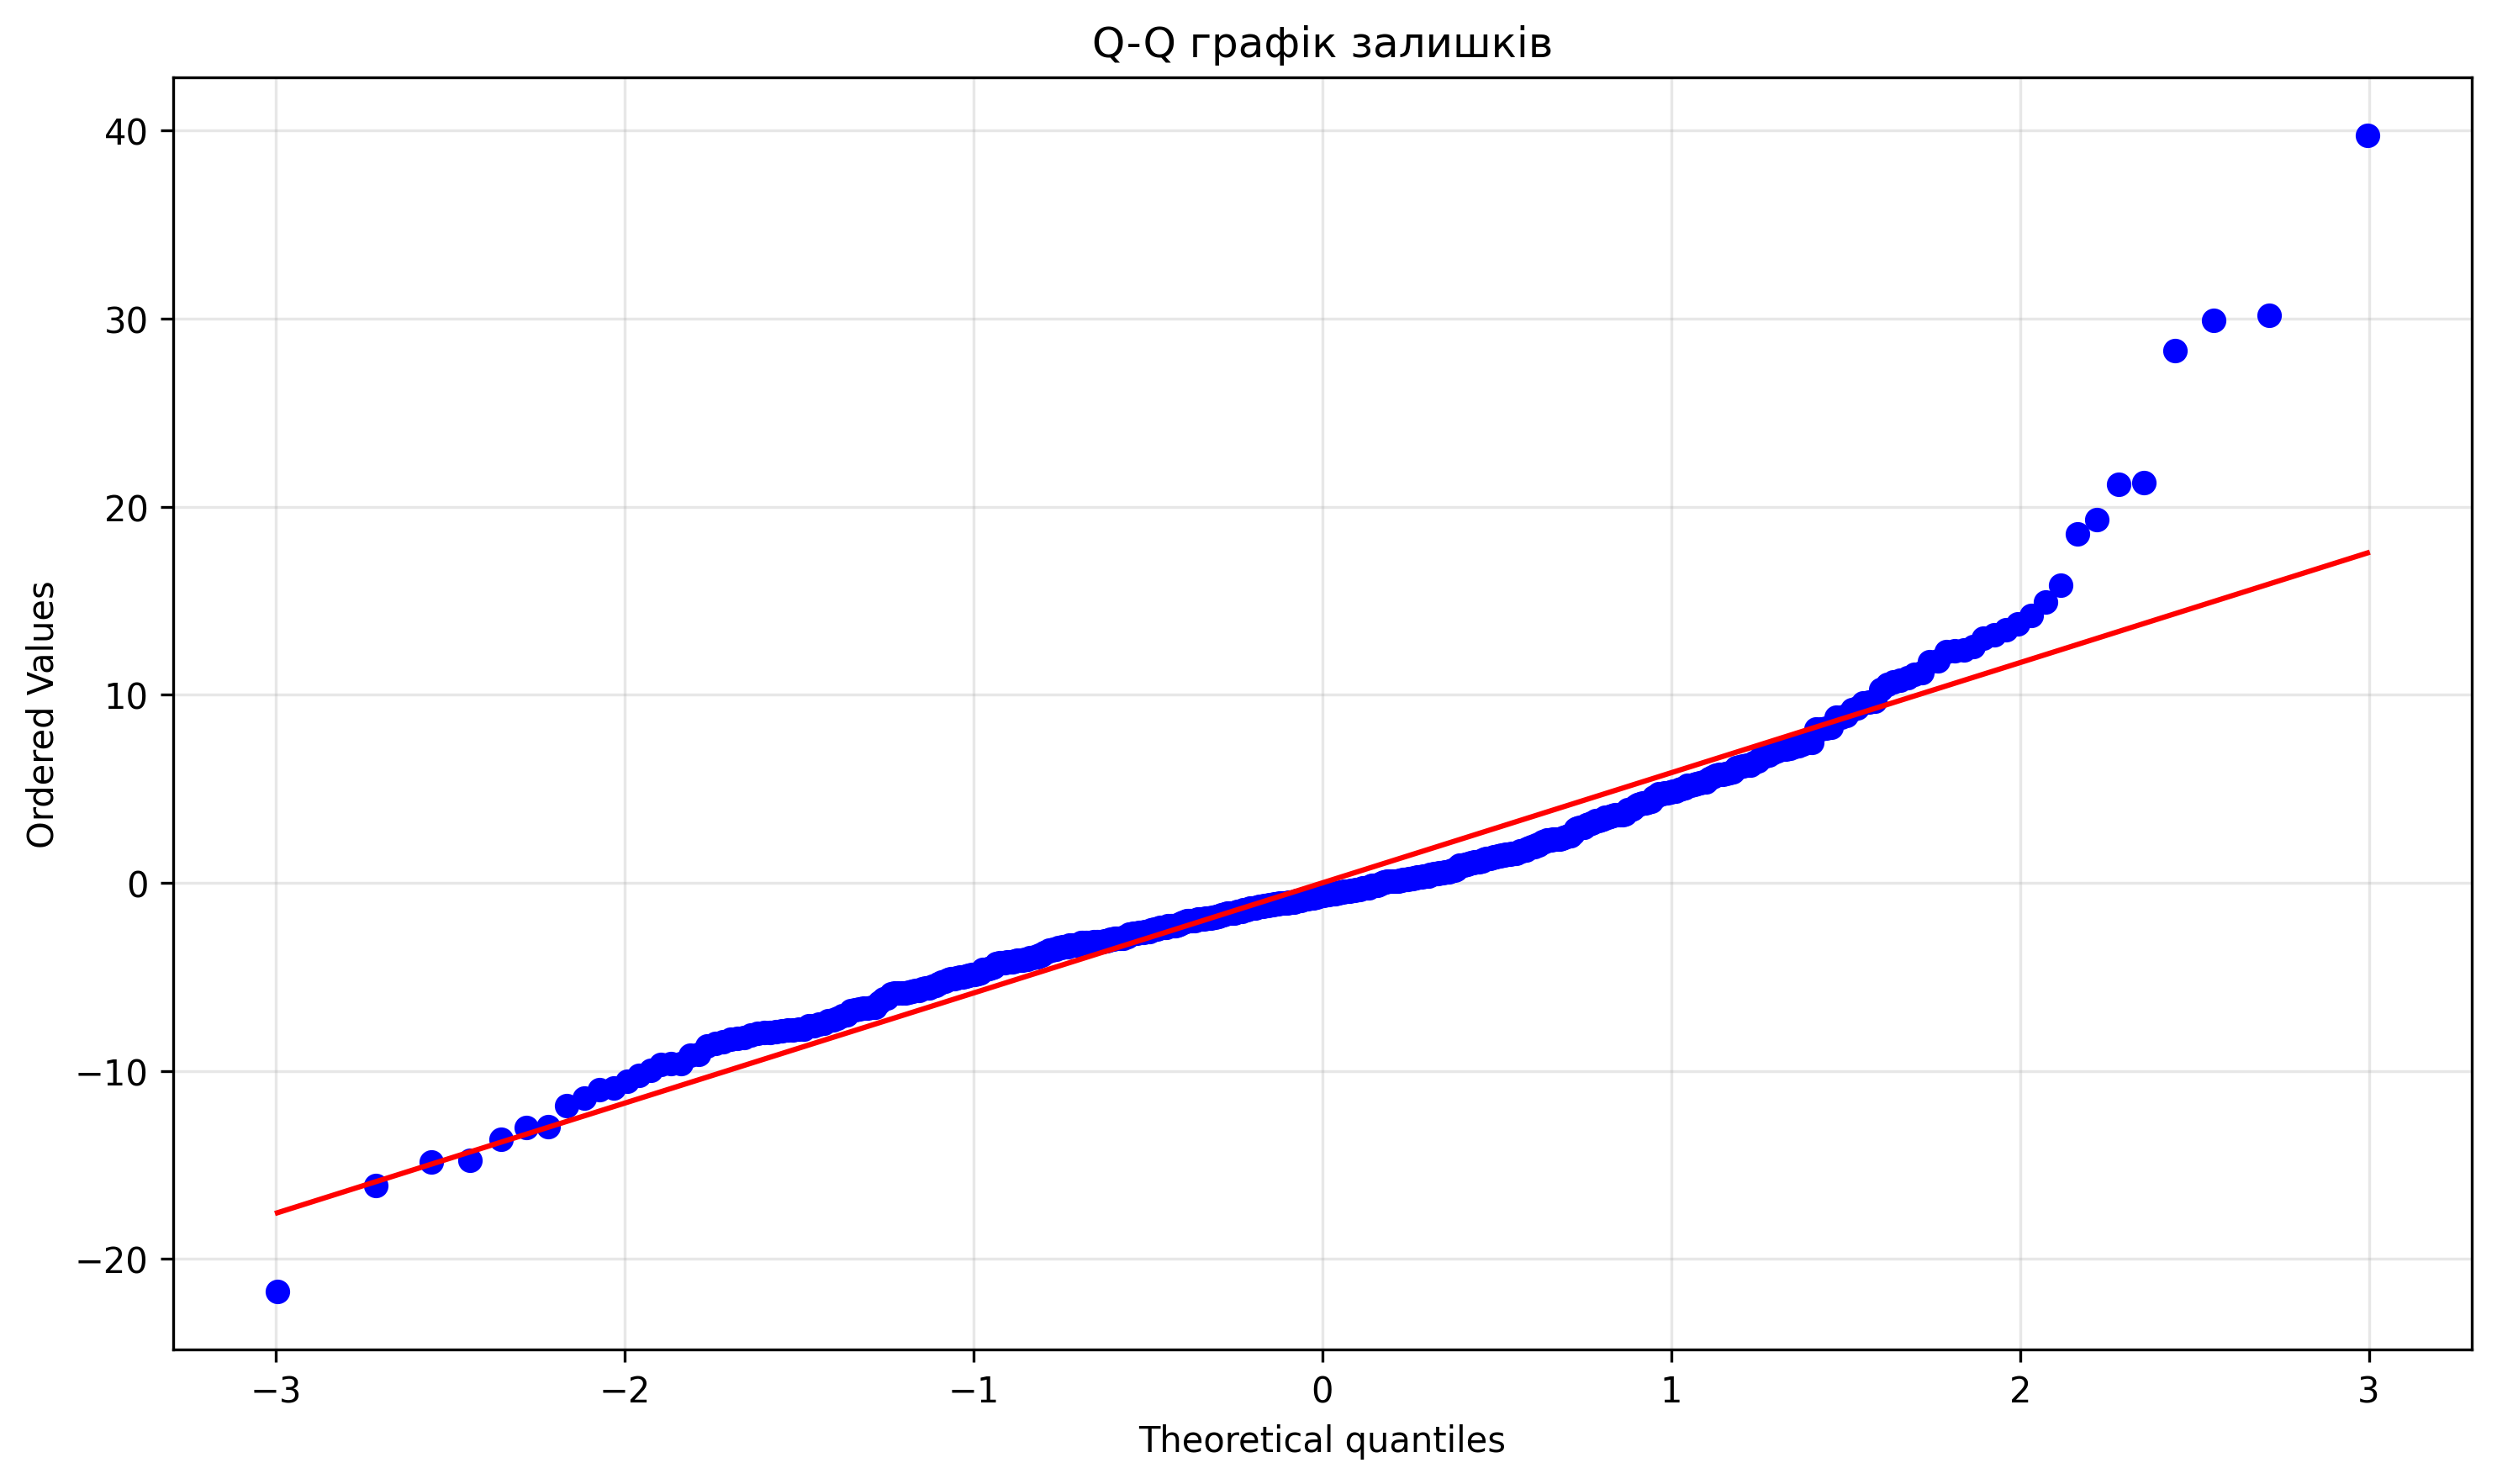
\includegraphics[width=0.8\textwidth]{qq_plot.png}
        \caption{Нормальний Q-Q графік залишків}
        \label{fig:нормальний_q-q_графік_залишків}
    \end{figure}

    \vspace{0.5cm}
    
    \begin{figure}[H]
        \centering
        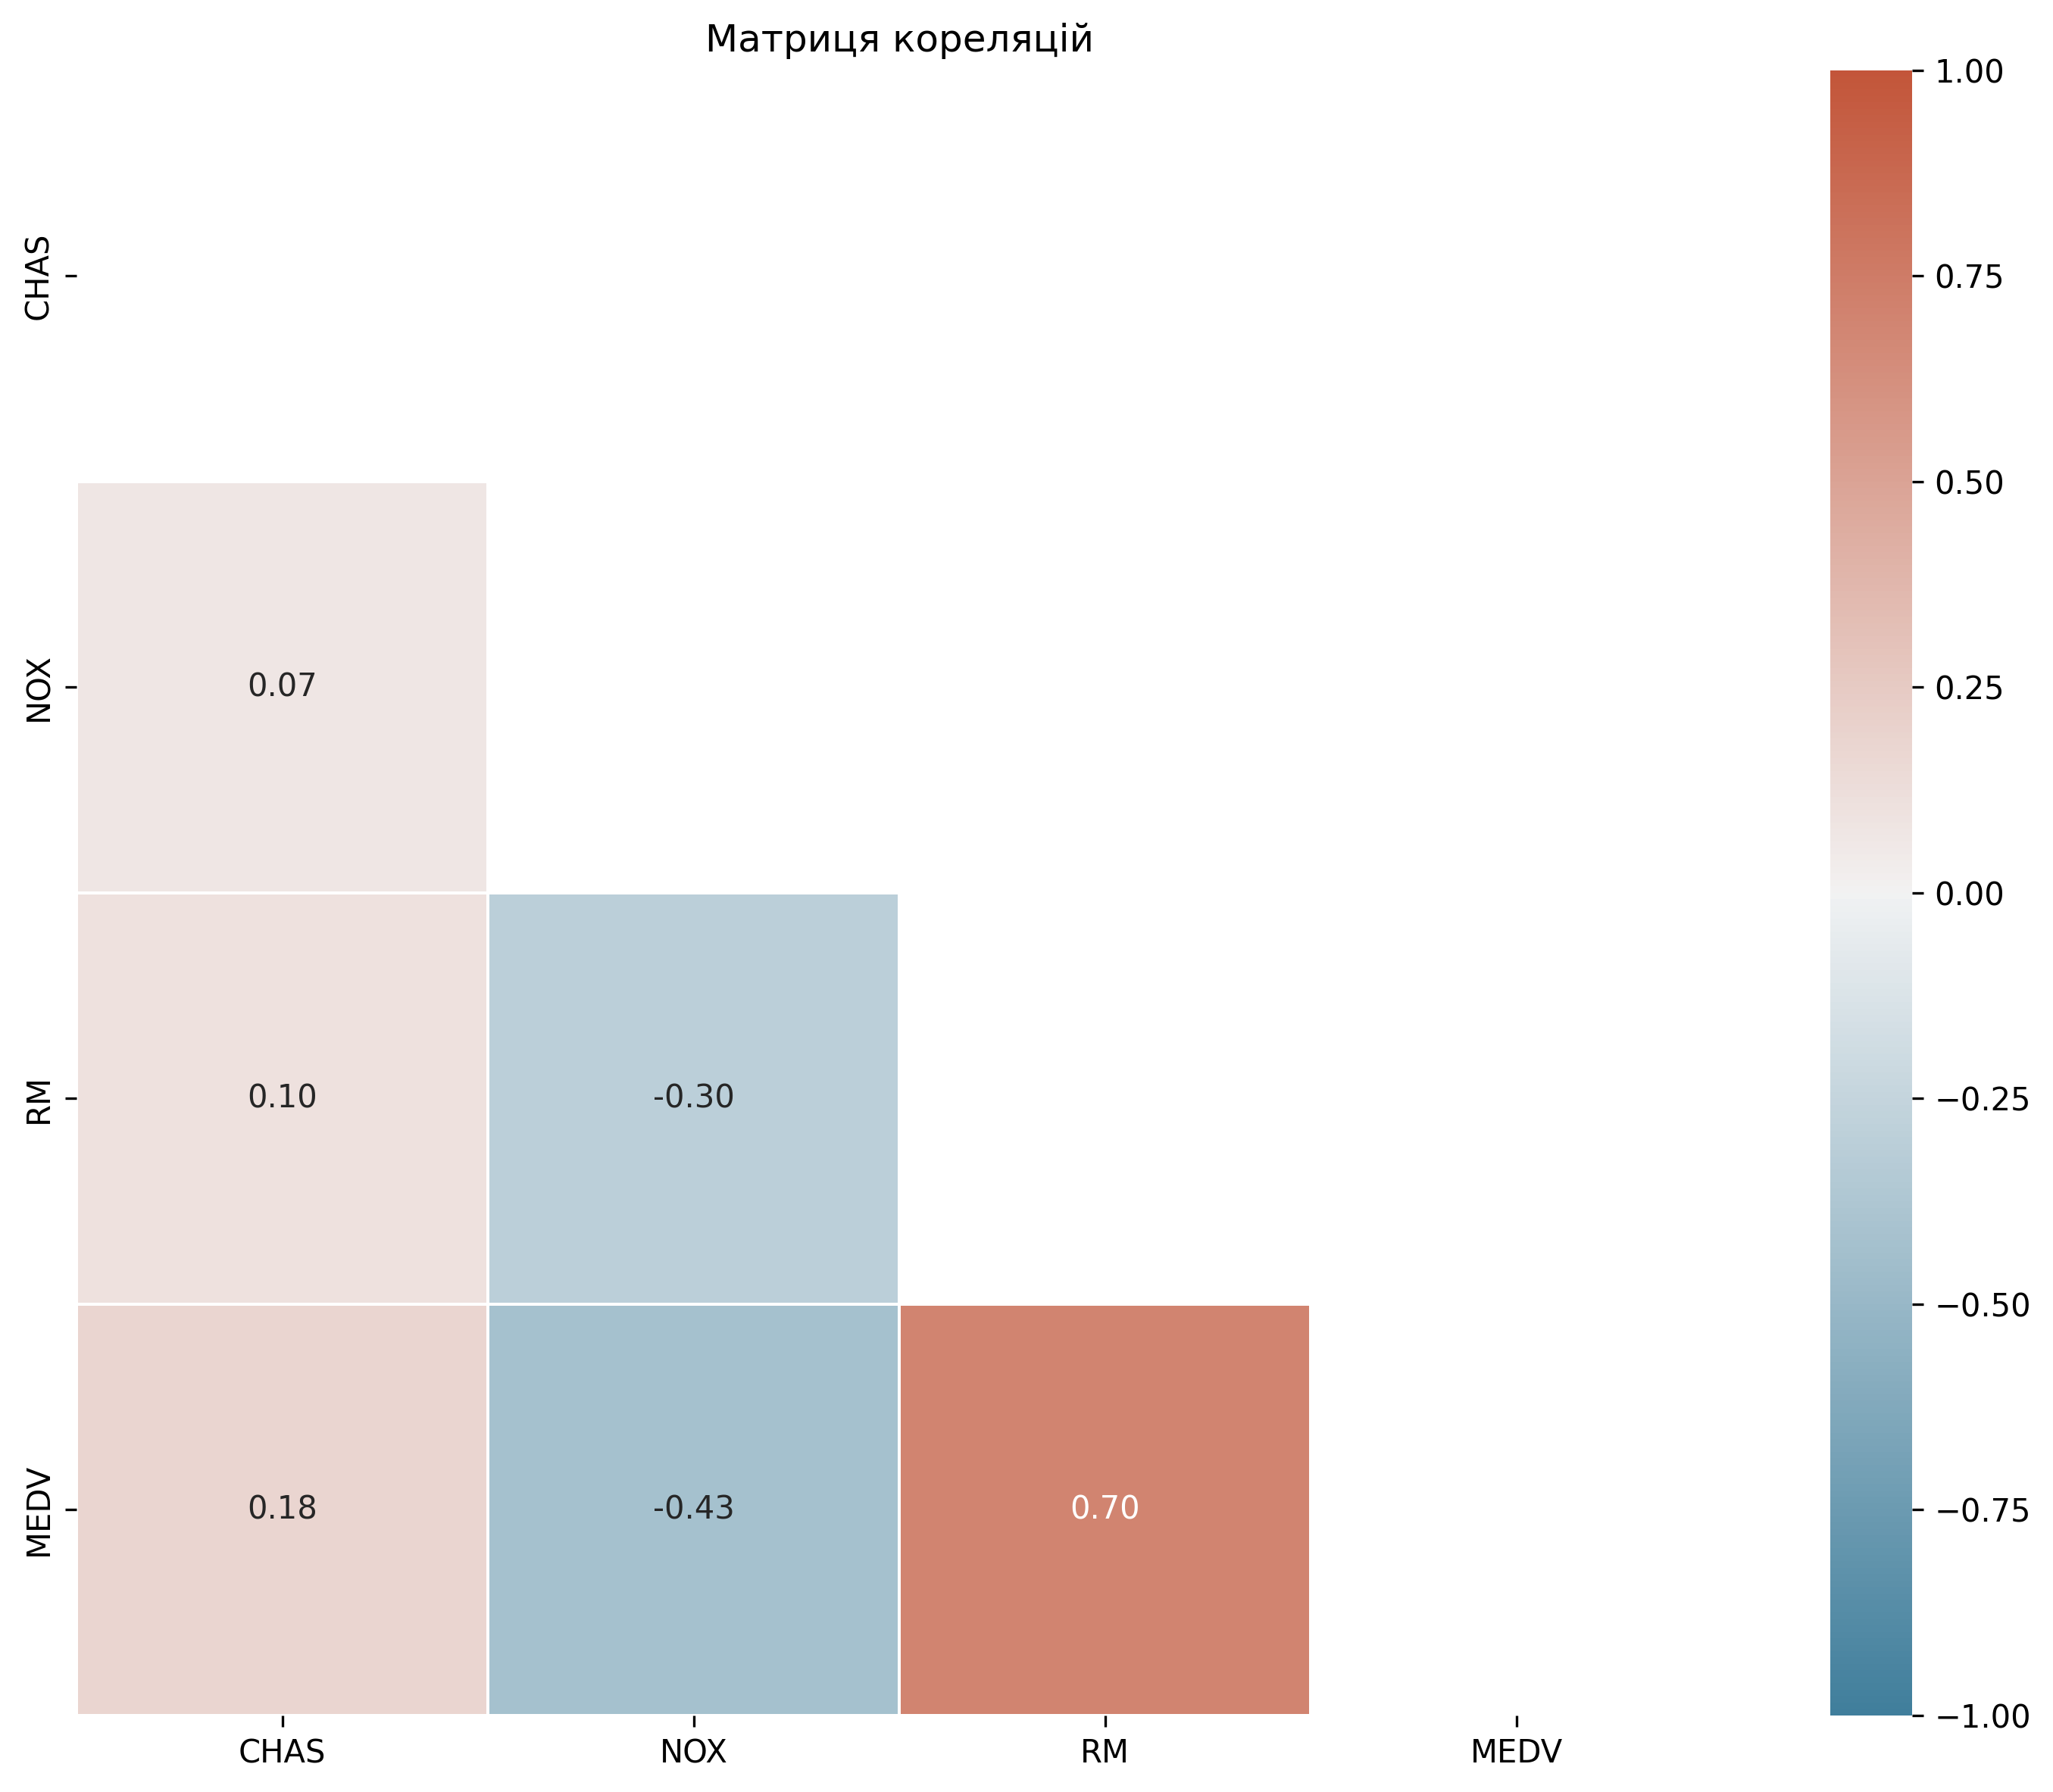
\includegraphics[width=0.8\textwidth]{correlation_heatmap.png}
        \caption{Теплова карта кореляцій}
        \label{fig:теплова_карта_кореляцій}
    \end{figure}

    \vspace{0.5cm}
    
    \begin{figure}[H]
        \centering
        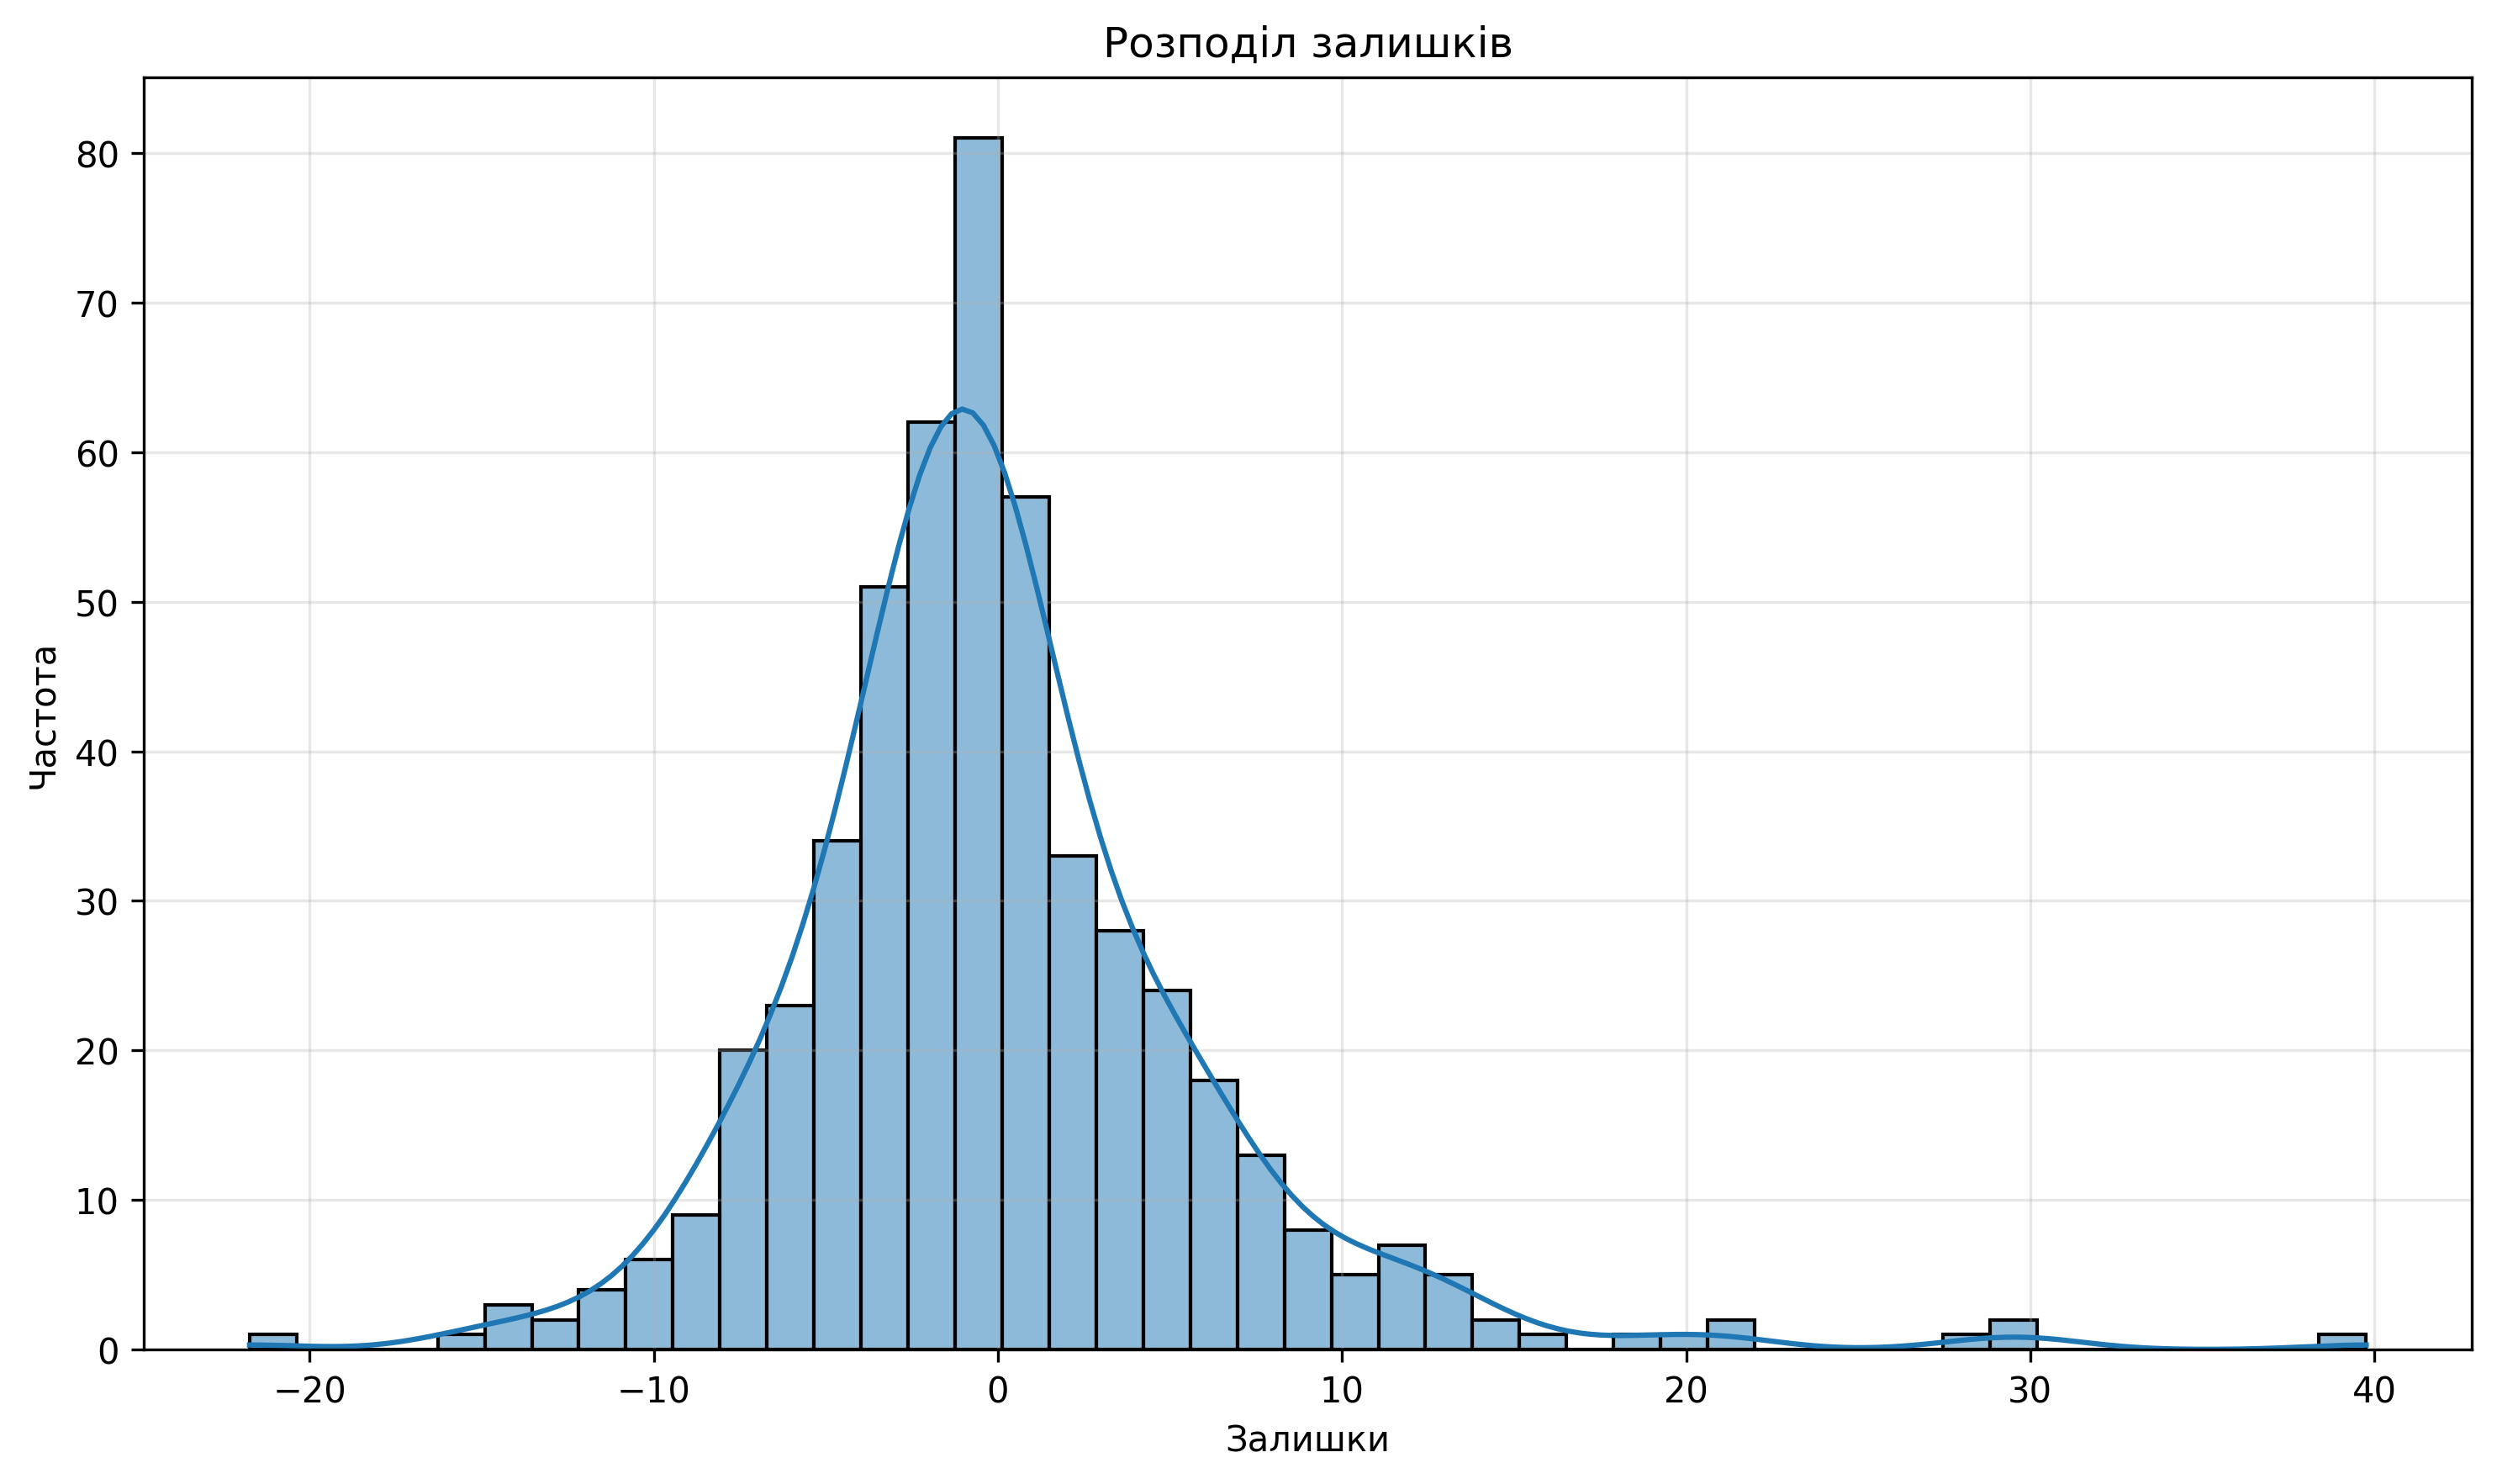
\includegraphics[width=0.8\textwidth]{residuals_hist.png}
        \caption{Гістограма залишків}
        \label{fig:гістограма_залишків}
    \end{figure}

    \vspace{0.5cm}
    
    \section{Кореляційна матриця}

    \begin{center}
    \begin{tikzpicture}
    \matrix (m) [matrix of nodes, nodes={align=center, text width=3em}, 
                 row sep=-\pgflinewidth, column sep=-\pgflinewidth,
                 nodes in empty cells,
                 row 1/.style={nodes={font=\bfseries}},
                 column 1/.style={nodes={font=\bfseries}},
                 every node/.style={text height=1em, text depth=.5em,
                                   text centered, minimum width=3em, minimum height=2em}
                ] {
     & CHAS & NOX & RM & MEDV \\
CHAS & \textcolor{blue}{1.00} & 0.07 & 0.10 & 0.18 \\
NOX & 0.07 & \textcolor{blue}{1.00} & -0.30 & -0.43 \\
RM & 0.10 & -0.30 & \textcolor{blue}{1.00} & 0.70 \\
MEDV & 0.18 & -0.43 & 0.70 & \textcolor{blue}{1.00} \\

    };
    \draw (m-1-1.north west) -- (m-1-5.north east);
    \draw (m-1-5.north east) -- (m-5-5.south east);
    \draw (m-5-5.south east) -- (m-5-1.south west);
    \draw (m-5-1.south west) -- (m-1-1.north west);
    \draw (m-1-1.north west) -- (m-1-5.north east);
    \draw (m-1-5.north east) -- (m-5-5.south east);
    \draw (m-5-5.south east) -- (m-5-1.south west);
    \draw (m-5-1.south west) -- (m-1-1.north west);
    \draw (m-2-1.south west) -- (m-2-5.south east);
    \draw (m-1-2.north east) -- (m-5-2.south east);
    \end{tikzpicture}
    \end{center}

    \vspace{0.5cm}

    \section{Інтерпретація результатів}

    Дана модель багатофакторної лінійної регресії показує залежність змінної \textbf{MEDV} від змінних \textbf{CHAS}, \textbf{NOX}, \textbf{RM}.

    Коефіцієнт детермінації $R^2$ дорівнює 0.5537, що означає, що 55.4\% варіації залежної змінної пояснюється включеними у модель незалежними змінними.

    Середньоквадратична похибка (MSE) становить 37.6753, що є мірою середнього квадратичного відхилення спостережуваних значень від передбачених.

    \vspace{0.5cm}

    \section{Висновки}

    Результати аналізу показують, що модель має помірну пояснювальну здатність.
    
    Найбільший вплив на залежну змінну мають фактори:
    \begin{itemize}
        \item \textbf{NOX}: зменшує значення залежної змінної на 20.2150 одиниць при зміні на одну одиницю
    \item \textbf{RM}: збільшує значення залежної змінної на 7.9116 одиниць при зміні на одну одиницю
    \item \textbf{CHAS}: збільшує значення залежної змінної на 5.0253 одиниць при зміні на одну одиницю

    \end{itemize}
    
    \end{document}
    